\chapter{Introdução a Estatística}
\section{Aspectos Históricos}

\inic Desde o começo da civilização que a estatística tem estado
sempre presente, nos primórdios mais oculta e na atualidade mais
visível. o primeiro dado estatístico disponível foi o de registros
egípicios sobre presos de guerra que datam de 5000 a.C (MEMÓRIA, 2004).\vskip0.3cm 

Há indícios de que 3000 anos a.C. existem também registros egípicios
de falta de mão-de-obra relacionada a construção de pirâmides,
conforme evidenciam pesquisas arqueológicas. \vskip0.3cm 

No 4o. livro do Velho
Testamento faz referência à uma instrução dada a Moisés, para que
fizesse um levantamento dos homens de Israel que estivessem aptos
para guerrear. Confúcio relatou que no ano de 2238 a.C o imperador
da China Yao, ordenou que fosse feito o primeiro recenseamento com
fins agrícolas e comerciais . Desses registros também se utilizaram
as civilizações pré-colombianas dos Maias, Incas e
Astecas (LOPES \& MEIRELES, 2005) e (BAYER et al, 2009).\vskip0.3cm


No japao o primeiro recenseamento surgiu em 86 a.C, no tempo do Imperador Soujin, onde as atividades da população eram registradas para examinar a sua evolução.\vskip0.3cm


Na era cristã, o governador da Síria, Quirino, que incluía a Judéia
e a Galilélia, por ordem do senado, teve que fazer um
recenseamento no qual as pessoas tinham que ser entrevistadas no
local de origem. Acredita-se que, não fosse a Estatística Jesus
Cristo não teria nascido numa manjedoura em Belém e a história do
cristianismo, e quase toda a cultura ocidental, poderia ter sido
diferente. \vskip0.3cm


Como está escrito na Bíblia, no Novo Testamento, Lucas
cap. 2:1-2, o imperador Augusto mandou uma ordem para todos os
povos do império, dos quais, todas as pessoas deviam se registrar
para que fosse feita uma contagem da população. Foi então que, São
José e a Virgem Maria saíram de Nazareth, na Galiléia, para Belém,
na Judéia, para responder ao censo ordenado pelo imperador César
Augusto. Assim, foi enquanto estavam na cidade que Jesus
Nasceu. Um acontecimento ao acaso, mas, se o desfecho fosse diferente, se não fosse a estatística relacionada a contagem da população, a história da religião católica poderia ser outra.(MEMORIA, 2004) e (LOPES \& MEIRELES, 2005).\vskip0.3cm



Com o Renascimento, foi despertado o interesse pela coleta de
dados estatísticos, principalmente por suas aplicações na
administração pública. A Igreja Católica Romana tornou compulsório, a partir do Concílio de Trento (1545-1563), a importância dos
registros de batismos, casamentos e óbitos (MEMÓRIA,
2004).\vskip0.3cm

%Em 620 surgiu na cidade de Constantinopla o primeiro Bureau de
%Estatística.\vskip0.3cm

%\newpage

Desde a remota antiguidade, os governos têm se interessado por
informações sobre suas populações e riquezas, tendo em vista,
principalmente, fins militares e tributários. O registro de
informações perde-se no tempo (MEMÓRIA, 2004).\vskip0.3cm


Não é tarefa fácil saber quando se originou a história de qualquer
ramo do conhecimento, pois isso vai depender do conceito que
fizermos dele e que, naturalmente, evoluirá no decorrer do tempo.
A história da Estatística bem confirma esta asserção (MEMORIA,
2004).\vskip0.3cm

As primeiras aplicações da estatística estavam voltadas para as
necessidades de Estado, na formulação de políticas públicas,
fornecendo dados demográficos e e\-co\-nô\-mi\-cos à administração
pública. A abrangência da estatística aumentou no começo do século
XIX para incluir a acumulação e análise de dados de maneira geral.
Hoje, a estatística é largamente aplicada nas ciências naturais, e
sociais, inclusive na administração pública e privada.\vskip0.3cm

Seus fundamentos matemáticos foram postos no século XVII com o
desenvolvimento da teoria das probabilidades por Pascal e Fermat,
que surgiu com o estudo dos jogos de azar. O uso de computadores
modernos tem permitido a computação de dados estatísticos em larga
escala e também tornaram possível novos métodos antes
impraticáveis.\vskip0.3cm


Contudo, mesmo que a prática de coletar dados sobre colheitas,
composição da população humana ou de animais, impostos, etc.,
fosse conhecida pelos egípcios, hebreus, caldeus e gregos, e se
atribuam a Aristóteles cento e oitenta descrições de Estados,
apenas no século XVII a Estatística passou a ser considerada
disciplina autônoma, tendo como objetivo básico a descrição dos
Bens do Estado.\vskip0.3cm


%Raríssimos são os ramos do conhecimento e as atividades humanas que
%podem dispensar o apoio de técnicas estatísticas em seu desenvolvimento.
%Um olhar mais acurado em torno de quase todos os fenômenos que nos cercam nos remete à conclusão de que tais técnicas estão participando cada vez mais do nosso cotidiano. Essa tendência parece se tornar mais acentuada na medida em que se expandem os recursos oferecidos pela informática, já que eles facilitam sobremaneira a análise de dados. Se antes o conhecimento estatístico era privilégio daqueles que tinham inclinação vocacional para lidar com números, hoje se tornou requisito fundamental no exercício de várias profissões (CORRAR et at., 2007).\vskip0.3cm



A utilização da Estatística é cada vez mais acentuada em qualquer atividade profissional da vida moderna. Nos seus mais diversificados ramos de atuação, as pessoas estão freqüentemente expostas à Estatística, utilizando-a com maior ou menor intensidade. Isto se deve as múltiplas aplicações que os métodos estatísticos proporcionam aqueles que dele necessitam. O uso de estatísticas é fundamental em qualquer área de atividade. São elas que permitem identificar os principais problemas, definir prioridades e avaliar o resultado dos trabalhos executados.\vskip0.3cm


\section{Etimologia: Estatística e Censo}

\inic O termo estatística deriva do neolatim statisticum collegium
("Conselho de Estado") e do Italiano statista ("estadista" ou
"político"). O alemão Statistik, introduzido pelo primeira vez por
Gottfried Achenwall (1749), professor da Universidade de
Gottingen, designava originalmente a análise de dados sobre o
Estado, significando a "ciência do Estado" (então chamada
aritmética política (political arithmetic) em inglês). 

\vspace{-6.0cm}
\begin{figure}
\centering
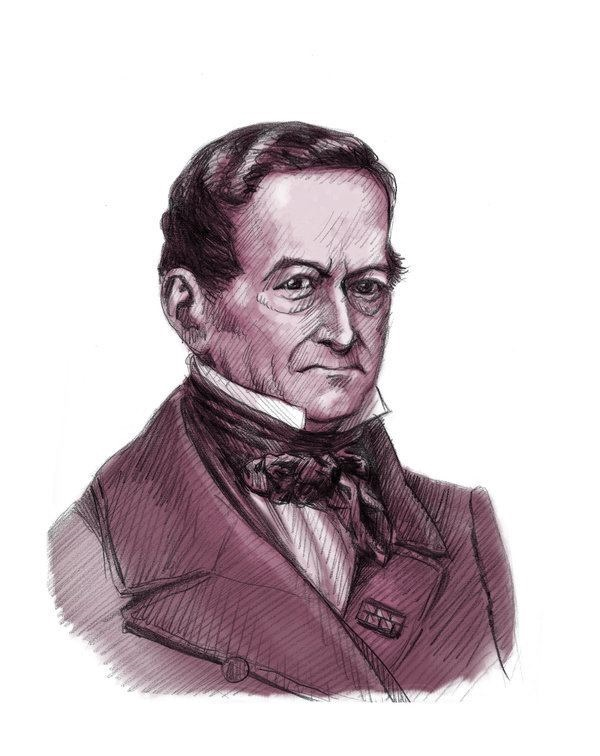
\includegraphics[scale=0.4]{figures/gottfried_achenwall.jpeg}
\vspace{-0.2cm}
\caption{Gottfried Achenwall(1719- 1772)}
\label{fig:my_label8}
\end{figure}






A palavra adquiriu o significado de coleta e classificação de dados em geral
através de Sir John Sinclair. Assim, o propósito original da
Statistik era fornecer os dados a serem usados pelo governo e
outras organizações. A coleta de dados sobre estados e localidades
continua, em grande parte através de órgãos estatísticos nacionais
e internacionais. Em particular, os censos fornecem informação
regular sobre as populações (STIGLER, 1990).\vskip0.3cm

\inic A palavra "CENSO" é derivada da palavra "CENSERE", que em Latim
significa "TAXAR". Em 1085, Guilherme, O Conquistador Normando,
solicitou um levantamento estatístico da Inglaterra, que deveria
conter informações sobre terras, proprietários, uso da terra,
empregados e animais, dos conquistados anglo-saxões. Os resultados
deste Censo foram publicados em 1086 no livro intitulado "Domesday
Book" e serviram de base para o cálculo de impostos. Na Enciclopédia Britânica, o verbete "STATISTICS" apareceu em 1797 (STIGLER, 1990).



\section{Formação da Estatística no Brasil}

\inic Um dos registros mais antigos sobre a introdução da Estatística no Brasil é uma
carta régia, datada de 8 de julho de 1800, onde o rei D. João VI solicita ao vice-rei do
Estado do Brasil a remessa de dados censitários do Brasil ao reino de Portugal.\vskip0.3cm


\inic Em 1808, D. João VI criou, a primeira instituição brasileira de ensino superior de tipo técnico, a Academia Real da Marinha, na cidade do Rio de Janeiro. Dois anos depois, é criada também a Academia Real Militar, destinada a formar oficiais da classe de engenheiros, geógrafos e
topógrafos. Nessas instituições, o ensino de disciplinas de ciências exatas seria, enfim,
encorajado no Brasil, inicialmente com as disciplinas de Física, Matemática e Química,
e posteriormente com a Estatística.\vskip0.3cm


\inic No ano de 1872, houve o primeiro censo geral da população
brasileira feito por José Maria da Silva Paranhos, conhecido como
Visconde do Rio Branco (1819-1880).\vskip0.3cm 


\inic Em 1934, foi criada a Faculdade de Filosofia, Ciências e Letras - FFCL da Universidade de São Paulo – USP, nascendo a cadeira de Estatística Geral e Aplicada pertencentes aos cursos oriundos das Ciências Sociais e Pedagogia (PEREIRA e MORETTIN, 1991).\vskip0.3cm

\inic Em 1936, tem-se a criação do Instituto Brasileiro de Geográfia e Estatística (IBGE), tornandos-se o Orgão máximo de todas as atividades estatísticas, que envolvem a sociedade Brasileira.\vskip0.3cm

\inic Em meados de 1946, a Faculdade de Filosofia, Ciências e Letras - FFCL da Universidade de São Paulo – USP, regulamentou a primeira turma de Pós-graduação em Estatística do Brasil (LOPES, 1988).\vskip0.3cm


\inic Em 1953 duas escolas iniciaram o ensino de estatística no brasil: uma no
Rio de Janeiro, a Escola Nacional de Ciências Estatística (ENCE) e
a outra conhecida como Escola de Estatística da Bahia. Só em 1972
que surge o primeiro computador brasileiro, que ajudou a dar um
grande salto na estatística.\vskip0.3cm


\inic A inclusão da Estatística no Ensino Fundamental e Médio apareceu a
partir da determinação dos Parâmetros Curriculares Nacionais
(PCN's) em 1997. De acordo com os PCN's o ensino da estatística na
escola vem ao encontro de uma sociedade que, muitas vezes, se
comunica através de gráficos, tabelas, estatísticas do trânsito,
da saúde, do jogo de futebol, etc. Assim, para que o cidadão
sobreviva e assimile este mar de estatística é necessário que
alguns conceitos sejam trabalhados desde a escola.


\section{Conceitos Fundamentais}

\subsection{Definição de Estatística}

\inic É extremamente difícil definir a Estatística. O número de definições
que se encontram é extremamente grande, tendo em vista que seu domínio é
muito amplo. Assim, listam-se algumas definições formais acerca do que
seria o conceito de Estatística.\vskip0.3cm

Segundo Rao (1973), a estatística pode ser definida de uma forma
simples e objetiva. Ele define a estatística pela equação:

\begin{center}
Conhecimento Incerto + Conhecimento Sobre A Incerteza =
 Conhecimento Útil
\end{center}

Neste sentido, o objetivo da Estatística é analisar os dados
disponíveis e que estão sujeitos a um certo grau de incerteza no
planejamento e obtenção de resultados (RAO, 1999).\vskip0.3cm


Segundo Stein \& Loesch (2008), a estatística é a ciência que se
preocupa com a coleta, organização, apresentação, interpretação e
análise de dados amostrais extraídos de uma determinada
população.\vskip0.3cm

O dicionário Aurélio (2005) definiu a estatística como uma parte da matemática em que se investigam os processos de obtenção, organização e análise de dados sobre uma população ou coleção de seres quaisquer, e os métodos de tirar conclusões e fazer predições com base nesses dados.\vskip0.3cm

De acordo com Motta \& Wagner (2003), a estatística é o ramo do conhecimento que se destina ao estudo dos processos de obtenção, coleta, organização, apresentação, análise e interpretação dos dados numéricos ou variáveis referentes a qualquer fenômeno, sobre uma população ou amostra.\vskip0.3cm

É possível distinguir duas concepções para a palavra ESTATÍSTICA: no plural (estatísticas), indica qualquer coleção de dados numéricos, reunidos com a finalidade de fornecer informações acerca de uma atividade qualquer. Assim, por exemplo, as estatísticas demográficas referem-se aos dados numéricos sobre nascimentos, falecimentos, matrimônios, desquites, etc. As estatísticas econômicas consistem em dados numéricos relacionados com emprego, produção, vendas e com outras atividades ligadas aos vários setores da vida econômica. No singular (Estatística), indica a atividade humana especializada ou um corpo de técnicas, ou ainda uma metodologia desenvolvida para a coleta, a classificação, a apresentação, a análise e a interpretação de dados quantitativos e a utilização desses dados para a tomada de decisões.\vskip0.3cm

O mundo está repleto de problemas. Para resolvermos a maioria deles, necessitamos de informações. Mas, que tipo de informação Que quantidade de informações? Após obtê-las, que fazer com elas? A Estatística trabalha com essas informações, associando os dados ao problema, descobrindo como e o que coletar de dados, assim capacitando o pesquisador (ou profissional ou cientista) a obter conclusões a partir dessas informações, de tal forma que possam ser entendidas por outras pessoas. Portanto, os métodos estatísticos auxiliam o cientista social, o economista, o engenheiro, o biólogo, o agrônomo e muitos outros profissionais a realizarem o seu trabalho com mais eficiência.\vskip0.3cm

Assim, uma igualdade que pode sintetizar as considerações descritas anteriormente sobre a estatística pode ser expressa como (PADOVANI, 2012):

\begin{center}
\fcolorbox{verdemar}{green}{ESTATÍSTICA} = \fcolorbox{verdemar}{green}{CIÊNCIA} + \fcolorbox{verdemar}{green}{TECNOLOGIA} + \fcolorbox{verdemar}{green}{ARTE}
\end{center}

A estatística se divide didaticamente em duas partes: Descritiva e Inferencial


\subsection{Estatística Descritiva, Dedutiva ou Analítica}

\inic É comum o profissional ou pesquisador defrontar-se com a situação de dispor de tantos dados que se torna difícil absorver completamente a informação que está procurando investigar. Com isso, se torna extremamente difícil captar intuitivamente todas as informações que os dados contêm, sendo necessário, portanto, que as informações sejam reduzidas até o ponto em que se possa interpretá-las mais claramente.\vskip0.3cm

A Estatística Descritiva é um ramo da estatística que aplica várias técnicas para descrever e sumariar um conjunto de dados.\vskip0.3cm

Stein \& Loesch (2008) definem a estatística descritiva como o nome dado ao conjunto de técnicas analíticas utilizadas para resumir certo conjunto de todos os dados coletados numa determinada investigação.\vskip0.3cm


É a parte da estatística que procura somente descrever e avaliar certo grupo de dados seja ele a população ou a amostra. Em estatística descritiva têm-se dois métodos que podem ser usados para a apresentação dos dados: Métodos Gráficos e/ou Tabular e Métodos Numéricos, envolvendo apresentação de medidas estatísticas, entre outras.\vskip0.3cm

%\newpage

O objetivo da Estatística Descritiva é o de representar de uma forma concisa, sintética e compreensível, a informação contida num conjunto de dados. Esta tarefa, que adquire grande importância quando o volume de dados for grande, concretiza-se na elaboração de tabelas e de gráficos, e no cálculo de medidas ou indicadores que representam convenientemente a informação contida nos dados.\vskip0.3cm


 A descrição dos dados também tem como objetivo identificar anomalias, até mesmo resultante do registro incorreto de valores, e dados dispersos, aqueles que não seguem a tendência geral do restante do conjunto. Não só nos artigos técnicos direcionados para pesquisadores, mas também nos artigos de jornais e revistas escritos para o público leigo, é cada vez mais freqüente a utilização destes recursos de descrição para complementar a apresentação de um fato, justificar ou referendar um
 argumento.\vskip0.3cm

 %\newpage

 Ao se condensar os dados, perde-se informação, pois não se têm as observações originais. Entretanto, esta perda de informação é pequena se comparada ao ganho que se tem com a clareza da interpretação proporcionada. Ao mesmo tempo que o uso das ferramentas estatísticas vem crescendo, aumenta também o abuso de tais ferramentas. É muito comum vermos em jornais e revistas, até mesmo em periódicos científicos, gráficos voluntariamente ou intencionalmente enganosos e estatísticas obscuras para justificar argumentos polêmicos.





\subsection{Estatística Indutiva, Amostral ou Inferencial}

\inic Usualmente, é impraticável observar toda uma população, seja pelo custo alto seja por dificuldades operacionais. Examina-se então uma amostra, de preferência bastante representativa, para que os resultados obtidos possam ser generalizados para toda a população. Um experimento pode ter por finalidade a determinação da estimativa de um parâmetro de uma função. Toda conclusão tirada por amostragem, quando generalizada para a população, apresentará um grau de incerteza. Ao conjunto de técnicas e procedimentos que permitem dar ao pesquisador um grau de confiabilidade nas afirmações que faz para a população, baseadas nos resultados das amostras, damos o nome de Inferência Estatística.\vskip0.3cm

A estatística indutiva ou inferencial é a parte da estatística que, baseando-se em resultados obtidos da análise de uma amostra da população, procura inferir, induzir ou estimar as leis de comportamento da população da qual a amostra foi retirada. Refere-se a um processo de generalização a partir de resultados particulares. É, portanto, a parte da estatística referente a conclusões sobre as fontes de dados (CASTANHEIRA, 2005).\vskip0.3cm

%\newpage

Por exemplo, suponha-se que deseja conhecer o grau de pureza de alumina a ser exportada por um navio no porto de Manaus. Como não se pode verificar esse grau de pureza em toda a população do minério, se pega uma parte como amostra e procedem-se na mesma os testes necessários. Suponha-se que o resultado obtido nesse teste é válido para toda a população.\vskip0.3cm

Esse processo de generalização, que é caracterizado do método indutivo, está associado a uma margem de incerteza. Esta incerteza de deve ao fato de que a conclusão, que se pretende obter para toda a população analisada, baseia-se em uma amostra do total de observações. A medida de incerteza é tratada mediante técnicas e métodos que se fundamentam na teoria das probabilidades.\vskip0.3cm


Em suma, para o estabelecimento de inferências ou conclusões sobre um grupo maior (no caso a população) precisa-se usar algo além do que será visto em Estatística Descritiva. Na verdade esse algo mais seria o uso de métodos estatísticos que caracterize a área da estatística conhecida como "Estatística Indutiva" ou "Inferência Estatística".\vskip0.3cm

A estatística inferencial pode ser classificada em:

\begin{enumerate}
  \item \textbf{Estimação de Parâmetros}: inferências sobre os parâmetros (descritores matemáticos como média, desvio-padrão, proporções, risco relativo, correlação, etc.) na população em estudo baseada em estatísticas análogas (estimadores dos parâmetros) obtidos a partir da amostra.
  \item \textbf{Teste de Significância}: as probabilidades são calculadas com base em hi\-pó\-te\-ses sobre a associação exposição-desfecho na população em estudo.
\end{enumerate}


\subsection{Fenômeno Estatístico}

\inic A palavra \textbf{fenômeno} segundo o dicionário Aurélio significa qualquer modificação operada nos corpos pela ação dos agentes físicos ou quimícos. Tudo que é percebido pelos sentidos ou pela consciência. Fato de natureza moral e social, tudo que o que é objeto de experiência possível que se pode manifestar no tempo e no espaço, segundo as leis do entendimento. Assim, o fenômeno tem características próprias, ocupa lugar no tempo, têm essência e é objeto do conhecimento científico. \vskip0.3cm   

\inic O \textbf{fenômeno estatístico} é qualquer evento que se pretenda analisar, cujo estudo seja possível a aplicação do método estatístico. São divididos em três grupos:

\begin{enumerate}
  \item \textbf{Fenômeno de Massa ou Coletivo}: são aqueles que não podem ser definidos por uma simples observação. A estatística dedica-se ao estudo desses fenômenos;
  \item \textbf{Fenômeno Individual}: são aqueles que irão compor os fenômenos de massa, ou seja, do campo experimental;
  \item \textbf{Fenômeno de Multidão}: quando as características observadas para a massa não se verificam para o particular. São aqueles os quais só agem causas acidentais. A mortalidade, por exemplo, é o caso típico de um fenômeno de multidão.
\end{enumerate}


\subsection{Experimento Aleatório}

\inic Experimentos aleatórios são aqueles que, repetidos em idênticas condições, produzem resultados diferentes. Embora não se sabe qual o resultado que irá ocorrer num experimento, em geral, consegue-se descrever o conjunto de todos os resultados possíveis que podem ocorrer. As variações de resultados, de experimento para experimento, são devidas a uma multiplicidade de causas que não se pode controlar, a qual denominou acaso.

\subsection{Dado Estatístico}

Dados descrevem Fenômenos (ou Processos) ou entidades que são objetos de estudo ou análise. Desta forma, dados correspondem a atributos que podem ser caracterizados de acordo com diferentes critérios, sendo considerado a matéria-prima sobre o qual o pesquisador irá aplicar os métodos estatísticos.\vskip0.3cm

Os dados geralmente são organizados no que chamamos de \textbf{Matriz de Dados} . Se você já viu dados em uma \textbf{Planilha}, isso é uma matriz de dados. As planilhas são talvez a forma mais comum de disponibilização dos dados (Broman e Woo 2017).\vskip0.3cm



Cada linha (horizontal) representa uma observação (também chamada de unidades observacionais , casos ou assuntos). Estes são os indivíduos ou itens na amostra.\vskip0.3cm

Cada coluna (vertical) representa uma variável, a característica ou coisa que está sendo medida. Pense nas variáveis como medidas que podem variar de uma observação para outra.



\subsection{História Estatística}

A maior parte da visualização de dados é feita para fins de comunicação. Temos uma visão sobre um conjunto de dados, temos um público potencial e gostaríamos de transmitir nossa visão ao nosso público. Para comunicar nossa visão com sucesso, teremos que apresentar ao público uma história clara e emocionante. \vskip0.3cm

A necessidade de uma história pode parecer perturbadora para cientistas, jornalistas e Agentes Públicos, que podem equipará-la a inventar coisas, dar uma guinada nas coisas ou exagerar nos resultados. No entanto, essa perspectiva perde o importante papel que as histórias desempenham no raciocínio e na memória.\vskip0.3cm

Os cientistas frequentemente sabem como visualizar dados sem serem grosseiramente enganosos. No entanto, eles podem não ter um senso de estética visual bem desenvolvido e podem, inadvertidamente, fazer escolhas visuais que prejudicam a mensagem desejada. Os designers, por outro lado, podem preparar visualizações que parecem bonitas, mas jogam rápido e solto com os dados. 

%(WILKE, 2019). 
\subsubsection{O Que é uma História Estatística}

Por conta própria, as estatísticas são apenas números. Eles estão em toda parte em nossa vida. Os números aparecem em histórias esportivas, relatórios sobre a economia, atualizações do mercado de ações, para citar apenas alguns. Para significar alguma coisa, seu valor para a pessoa na rua deve ser trazido à vida.\vskip0.3cm 

Uma história é um conjunto de observações, fatos ou eventos, verdadeiros ou inventados, que são apresentados em uma ordem específica para criar uma reação emocional no público.\vskip0.3cm 

Uma história estatística é aquela que não apenas recita dados em palavras. Ele conta uma história sobre os dados. Os leitores tendem a se lembrar de ideias com mais facilidade do que dos dados. Já, uma história estatística transmite uma mensagem que conta aos leitores o que aconteceu, quem fez, quando e onde aconteceu e, esperançosamente, por que e como aconteceu.\vskip0.3cm 


Uma História Estatística pode:

\begin{itemize}
    \item Fornecer conhecimento geral, algumas perspectiva, e um certo contexto;
    \item Informar o debate sobre algumas questões específicas.
\end{itemize}


Em termos jornalísticos, o número por si só não é a história. Uma história estatística mostra aos leitores o significado, a importância e a relevância das informações mais atuais. Em outras palavras, responde à pergunta: por que meu público deveria querer ler sobre isso?\vskip0.3cm 

Finalmente, uma história estatística deve conter material digno de nota. Pergunte a si mesmo: a informação é suficientemente importante e inovadora para atrair a cobertura da mídia? A mídia pode escolher um foco diferente. Mas eles têm muitos outros fatores a considerar ao escolher um enredo.

Contar histórias estatísticas é sobre:

\begin{itemize}
    \item Chamar a atenção do leitor com um título ou imagem;
    \item Fornecer a história por trás dos números de forma fácil de entender, interessante e divertida;
    \item Encorajar leitores e outros a considerar como as estatísticas podem adicionar impacto a quase todas as histórias que eles têm para contar.
\end{itemize}

\subsubsection{Por Que Contar uma História Estatística}

Uma fonte estatística deve querer contar uma história sobre seus dados por pelo menos dois motivos.\vskip0.3cm 

Primeiro, o mandato da maioria das agências é informar o público em geral sobre a população, sociedade, economia e cultura da nação.\vskip0.3cm 

Essas informações orientarão os cidadãos na realização de seus trabalhos, na criação de suas famílias, nas compras e na tomada de muitas outras decisões.
Em segundo lugar, uma agência deve querer demonstrar a relevância de seus dados para o governo e o público.\vskip0.3cm 

Dessa forma, pode antecipar maior apoio público a seus programas, bem como melhorar o relacionamento com os entrevistados e maior visibilidade de seus produtos.\vskip0.3cm 

A maioria das agências conta principalmente com dois meios de comunicação de informações sobre as condições econômicas e sociais de um país e de seus cidadãos: a Internet e a Mídia.\vskip0.3cm 

A Internet tornou-se uma ferramenta importante para facilitar o acesso às informações da agência. Mais e mais membros do público acessam os dados de uma agência diretamente em seu site. Ainda assim, a maioria dos cidadãos obtém suas informações estatísticas da mídia e, de fato, a mídia continua sendo o principal canal de comunicação entre os institutos de estatística e o público em geral.\vskip0.3cm 


Uma maneira eficaz de um escritório de estatística se comunicar por ambos os meios é contar uma história estatística escrita da forma mais clara, concisa e simples possível. O objetivo da Internet é informar melhor o público por meio do acesso direto. Ao escrever para a mídia, o objetivo é obter uma cobertura positiva, precisa e informativa.\vskip0.3cm 

As estatísticas podem dizer às pessoas algo sobre o mundo em que vivem. Mas nem todo mundo é adepto de entender as estatísticas por conta própria. Consequentemente, as histórias estatísticas podem e devem fornecer uma ajuda.
Por último, mas não menos importante, a disponibilidade de estatísticas depende, em primeiro lugar, da cooperação voluntária dos respondentes da pesquisa. As agências estatísticas não podem confiar apenas em sua autoridade legal para garantir uma taxa de resposta adequada.\vskip0.3cm 


A disponibilidade de estatísticas também depende de até que ponto os entrevistados entendem que os dados servem a um propósito importante ao fornecer um espelho do mundo em que vivemos. Quanto mais uma agência estatística puder mostrar a relevância de seus dados, mais os entrevistados serão encorajados a fornecer os dados.\vskip0.3cm 

 As histórias estatísticas e os dados que elas contêm devem ser informativos e iniciar a discussão, mas nunca devem estar abertos à discussão. Em outras palavras, as informações devem ser precisas e a integridade da Fonte nunca deve ser questionada. As histórias devem ser baseadas em dados de alta qualidade que sejam adequados para descrever os problemas que abordam.\vskip0.3cm 

 As Fontes devem sempre garantir a confidencialidade dos dados de pessoas físicas ou jurídicas. Na verdade, as histórias estatísticas não podem identificar ou revelar de forma alguma dados sobre indivíduos ou empresas.\vskip0.3cm 





\subsection{Estatísticas Vitais}

As estatísticas vitais se baseiam em dados coletados de registros de eventos vitais, como nascimento e mortes. Assim, na area de saúde os profissionais precisam ser capazes de interpretar  estatísticas vitais a fim de diagnosticar e tratar pacientes de modo eficaz.








\subsection{Hipótese Estatística}

Em termos simples, uma \textbf{hipótese} é uma resposta possível de ser testada e fundamentada para uma pergunta feita relativa ao fenômeno escolhido. O pesquisador examina a literatura sobre ao fenômeno, obtêm a maior quantidade de conhecimento possível para responder ao problema formulado. Esta tentativa de resposta é a hipótese.\vskip0.3cm    

As hipóteses podem ser formuladas dependendo do tipo de problema, de três maneiras


\begin{enumerate}
\item \textbf{Hipóteses Univariadas}: são os que apresentam uma variável.  
\item \textbf{Hipóteses Multivariadas}: são os que apresentam ligação entre duas variáveis
\item \textbf{Hipóteses de Relação Casual}: são os que apresentam Relação de causa e efeito entre as variáveis.
\end{enumerate}


Existem algumas exigências para Formulação de Hipóteses:

\begin{itemize}
\item Formular hipóteses clara e precisas. Convêm estabelecer tanto as hipóteses de pesquisa, quanto as de nulidade.  
\item Indicar a importância e contribuição teórica das hipóteses.
\item Definir as variáveis, preferencialmente em termos operacionais, distinguindo as variáveis independentes e dependentes. 
\end{itemize}

A \textbf{hipótese estatística} é uma suposição formulada a respeito dos parâmetros de uma ou mais populações e é testada a partir dos resultados amostrais. As especificações sobre os parâmetros denominam-se Hipóteses Estatísticas, formuladas da seguinte forma:

\begin{itemize}
\item Hipótese Nula, da Nulidade ou Hipótese Básica, cujo o símbolo é representado da seguinte forma $H_{0}$ (Agá-zero).
\item Hipótese Alternativa, simbolizando como segue: $H_{1}$ ou $H_{A}$.
\end{itemize}

A hipótese de nulidade sempre significa \textbf{inocência}, ou seja, não há diferença entre os parâmetros das populações submetidas às observações ou aos experimentos. A hipótese alternativa sempre é \textbf{culpada}, de haver diferença entre os parâmetros dos universos em questão e contradiz a de nulidade.\vskip0.3cm



A hipótese nula é sempre a hipótese a ser examinada. As hipóteses estatísticas que podem ser testadas numericamente são utilizadas nos seguintes casos:

\begin{itemize}
\item testar a diferença entre dois ou mais grupos em relação a uma ou mais características.
\item testar a associação entre duas ou mais variaveis em um grupos ou entre vários grupos. 
\item testar a estimação de pontos das características de uma amostra ou população.
\end{itemize}


\newpage
\subsection{Tipos de Pesquisa Científica}

\inic Existem várias maneiras de classificar uma pesquisa, e os autores não são unânimes quanto à padronização desta classificação. Neste contexto, sugere-se uma maneira simples e objetiva.\vskip0.3cm 

\begin{quadro}[h!tp]
    \centering
    \caption{Equema geral dos Tipos de Pesquisas, segundo a sua classificação (IBGE, 2003).}
    \begin{tabular}{|l|l|}
    \hline \hline
    CLASSIFICAÇÃO                & TIPOS DE PESQUISAS   \\    
    \hline\hline
     Quanto à Finalidade         & Básica/Aplicada \\
     \hline
     Quanto à Natureza           & Observacional/Experimental  \\
     \hline
    Quanto à Forma de Abordagem  & Qualitativa/Quantitativa \\
    \hline
     Quanto aos Objetivos        & Exploratória/Explicativa \\
     \hline
    Quanto aos Procedimentos Técnicos     & Bibliográfica/Documental             \\
       \hline     
    Quanto ao Desenvolvimento    & Transversal/Longitudinal              \\
  \hline\hline
    \end{tabular}
    %\fonte{Autor: FONTELLES, 2011.}
\end{quadro}






\textbf{Quanto à Finalidade}: 

\begin{itemize}
\item \textbf{Pesquisa Básica ou Fundamental}: é aquela cujo objetivo é adquirir novos conhecimentos que possam contribuir para o avanço da ciência. Neste tipo de pesquisa, o investigador acumula conhecimentos e informações que podem, eventualmente, levar a resultados acadêmicos ou aplicados importantes. Alguns autores incluem, nesta categoria, as pesquisas realizadas na area acadêmica, aquelas realizadas na instituição de ensino superior como parte das atividades de ensino-aprendizagem, tal como nos trabalhos de conclusão de curso (KENDALL, 2003). 
\item \textbf{Pesquisa Aplicada ou Tecnológica}:é o tipo de pesquisa cujo objetivo é produzir conhecimentos científicos para aplicação prática voltada para a solução de problemas concretos, específicos da vida moderna. È a pesquisa que, além de produzir conhecimento, gera novos processos tecnológicos e novos produtos, com resultados práticos imediatos em termos econômicos e na melhoria da qualidade de vida (BOISSEL, 2004).
\end{itemize}

\textbf{Quanto à Natureza}: 

\begin{itemize}
\item \textbf{Pesquisa observacional}: O Pesquisador atua meramente como expectador de fenômeno ou fatos, sem, no entanto, realizar qualquer intervensão que possa interferir no curso natural e/ou no desfecho dos mesmos, embora possa, neste meio tempo, realizar medições, análises e outros procedimentos para coleta de dados (HULLEY et al, 2003).
\item \textbf{Pesquisa Experimental}: é qualquer pesquisa que envolve algum tipo de experimento. Neste caso, o pesquisador participa ativamente na condução do fenômeno, processo ou do fato avaliado, isto é, ele atua na causa, modificando-a, e avalia as mudanças no desfecho. Neste tipo de pesquisa, o investigador seleciona as variáveis que serão estudadas, define a forma de controle sobre elas e observa o efeitos sobre o objeto de estudo, em condições pré-estabelecidas. Assim, pelo fato das variáveis, ou da variável, poderem ser manipuladas pelo pesquisador, equívocos e vieses praticamente  desaparecem, sendo, por esta razão, considerada como o melhor tipo de pesquisa científica, pois proporciona maior confiabilidade em seus resultados. Os mais tradicionais tipos de delineamento da pesquisa experimental são os estudos controlados (duplo cego, randomizado ou aleatório, não-randomizado, autocontrolado e com controle externo) e não-controlados (SILVA, 2004). 
\end{itemize}


\textbf{Quanto á Forma de Abordagem}: 

\begin{itemize}
\item \textbf{Pesquisa Qualitativa}: é o tipo de pesquisa apropriada para quem busca o atendimento de fenômenos complexos específicos, em profundidade, de natureza social e cultural, mediante descrições, intepretações e comparações, sem considerar os seus aspectos numéricos em termos de regras matemácticas e estatísticas. Diferente da quantitativa, a pesquisa qualitativa é mais participativa, porém menos controlável e, por esta razão, tem sido questionada quanto a sua validade e confiabilidade (SILVA, 2001) e (SILVA, 2004).
\item \textbf{Pesquisa Quantitativa}: é aquela que trabalha com variáveis expressas sob a forma de dados numéricos e emprega rígidos recursos e técnicas estatísticas para classificá-los e análisá-los, tais como a porcentagem, a média, o desvio-padrão, o coeficiente de correlação e as regressões, entre outros. Em razão de sua maior precisão e coanfiabilidade, os estudos quantitativos são mais indicados para o planejamento de ações coletivas, pois seus resultados são passíveis de generalização, principalmente quando as amostras pesquisadas representam, com fidelidade, a população de onde retiradas (SILVA, 2001; SILVA, 2004).
\end{itemize}


\textbf{Quanto aos Objetos}: 

\begin{itemize}
\item \textbf{Pesquisa Exploratória}: este tipo de pesquisa visa a uma primeira aproximação do pesquisador com o tema, para torná-lo mais familiarizado com os fatos e fenômenos relacionados ao problema a ser estudado. No estudo, o investigador irá buscar subsídios, não apenas para determinar a relação existente, mas, sobretudo, para conhecer o tipo de relação (SILVA, 2011; SILVA, 2004) e (MARCONE, 2005).
\item \textbf{Pesquisa Explicativa}: tem por objetivo central explicar os fatores determinantes para a ocorrência de um fenômeno, processo ou fato, ou seja, visa explicar o porquê das coisas. É uma consequência lógica da pesquisa exploratória.(SILVA, 2011; SILVA, 2004) e (MARCONE, 2005).
\end{itemize}


\textbf{Quanto aos Procedimentos Técnicos}: 

\begin{itemize}
\item \textbf{Pesquisa Bibliográfica}: sua base é a analise de material já publicado. É utilizada para compor a fundamentação teórica a partir da avaliação atenta e sistemática de livros, periódicos, documentos, textos, mapas, fotos, manuscritos e, até mesmo, de material disponibilizado na internet etc. Este tipo de pesquisa fornece o suporte a todas as fases de um protocolo de pesquisa, pois auxilia na escolha do tema, na definição da questão da pesquisa, na determinação dos objetos, na formulação das hipóteses, na fundamentação da justificativa e na elaboração do relatório final.
\item \textbf{Pesquisa Documental}: é o tipo de pesquisa que tem o levantamento de documentos como base. É uma valiosa técnica de coleta de dados qualitativos. Assemelha-se à pesquisa bibliográfica, a qual utiliza a contribuição fornecida por diversos autores sobre um determinado assunto, enquanto na pesquisa documental, a coleta de informações é realizada em materiais que não receberam qualquer tipo de análise crítica. Neste tipo de pesquisa, os documentos consultados são, geralmente, classificados  como fontes primárias e fontes secundárias. No primeiro caso, são fontes cuja a origem remonta a época que se está pesquisando, ainda não analisados e que, frequentemente, foram produzidas pelas próprias pessoas estudadas, tais como correspondência, diários, textos literários e outros documentos mantidos em orgãos públicos e instituições privadas de qualquer natureza; no segundo, corresponde às fontes cujos trabalhos escritos se baseiam na fonte primária e tem como característica o fato de não produzir informações originais mas apenas uma análise, ampliação e comparação das informações contidas na fonte original.
\item \textbf{Pesquisa de Laboratório}: a principal característica é a sua realização em ambiente controlado, seja um laboratório ou não. Estas pesquisas, que geralmente são experimentais, adotam ambientes de simulação para reproduzir o fenômeno objeto do estudo, além de utilizar-se de instrumentos específicos e precisos de coleta e análise de material.
\item \textbf{Pesquisa de Campo}: uma pesquisa de campo procura coletar dados que lhe permitam responder aos problemas relacionados a grupos, comunidades ou instituições, com o objetivo de compreender os mais diferentes aspectos de uma determinada realizada, sendo mais frequentemente utilizada pelas áreas das ciências humanas e sociais mediante técnicas observacionais e com a utilização de questionários para a coleta de dados. 
\end{itemize}

\textbf{Quanto ao Desenvolvimento no Tempo}: 

\begin{itemize}
\item \textbf{Pesquisa Transversal e Longitudinal}: a diferença entre as duas é o intervalo de tempo que o pesquisador utiliza para a condução da pesquisa. No estudo transversal (ou seccional), a pesquisa é realizada em um curto período de tempo, em um determinado momento, ou seja, em um ponto no tempo, tal como agora, hoje. Mais dinâmica que a transversal, a pesquisa longitudinal pode ser classificada como prospectiva e retrospectiva e tem como subtipos o estudo caso-controle e o estudo de coorte prospectivo. 
\item \textbf{Pesquisa Prospectiva e Retrospectiva}: nesta classificação, a diferença é o sentido da condução da pesquisa em relação ao tempo de sua realização. Na pesquisa prospectiva, o estudo é conduzido a partir do momento presente e caminha em direção ao futuro. Já na retrospectiva, o estudo é desenhado para explorar fatos do passado, podendo ser delineado para retornar, do momento atual até um determinado ponto no passado.Um exemplo são os estudos caso-controle, em que o pesquisador pode marcar um ponto no passado e conduzir a pesquisa até o momento presente, pela  análise documental, tal como acontece no estudo do tipo coorte retrospectiva (coorte histórica). 
\end{itemize}



\subsection{População e Censo}

\begin{enumerate}
  \item \textbf{População ou Universo Amostral} : É o conjunto de todos os elementos relativos
  a um determinado fenômeno (ex: pessoas, animais, vegetais, ou objetos) que possuem ao menos uma característica em comum (de carater demográfico, clínico e temporal)
  entre todos os seus componentes , sendo um conjunto universo podendo ser
  finita ou infinita. Esta cacterística deve delimitar corretamente quais
  são os elementos da população que podem ser animados ou inanimados (SILVA, 2011).\vskip0.3cm

 As populações são classificadas segundo alguns critérios (AIRES, 2013).
 \begin{enumerate}
   \item \textbf{Tamanho}: finitas e infinitas;
   \item \textbf{Número de variáveis}: univariada, bivariadas e multivariadas;
   \item \textbf{Aspecto Existencial}: populações hipotéticas ou conceituais;
   \item \textbf{Objetivo da Investigação}: descritivo e analítico e combinado;
   \item \textbf{Obtenção dos Parâmetros}: censitários, inferenciais, alvo, emoldurado e de respondentes;
 \end{enumerate}



  \item \textbf{Censo} : É a coleta total das informações sobre a
  população em estudo, sendo realizado a cada 10 anos pelo Instituto
  Brasileiro de Geografia e Estatística (IBGE). A população é contada
  em todo o território do Brasil e os resultados são usados
  pelo governo no desenvolvimento de políticas públicas e na
  destinação dos fundos governamentais para as unidades federativas.
  Em 1872, foi realizado o primeiro Censo Nacional no Brasil, já o último foi em 2010.
\end{enumerate}

\subsection{Dados, Unidade, Amostra, Elemento e Amostragem}

\begin{enumerate}

\item \textbf{Dados Estruturados} : em que a informação se ajusta às estruturas
usuais de bases de dados, relativamente fáceis de armazenar e analisar.
Exemplos usuais de dados numéricos ou não, que podem ser dispostos
em matrizes de dados;

\item \textbf{Dados Não Estrturados}: tudo o que não se encaixa no item anterior, como arquivos de textos, páginas da web, emails, mídias sociais etc.

\item \textbf{Unidade} : É qualquer elemento individual da população;

\item \textbf{Amostra} : É uma parte ou subconjunto da população,
ou seja, são subconjuntos de elementos da mesma, de modo que
represente as características totais da população como se fosse
uma fotografia da mesma;

\item \textbf{Elemento} : O elemento sgnifica cada uma das
unidades observadas no estudo, no qual, após a determinação dos
elementos pergunta-se: o que fazer com estes? Pode-se medí-los,
observá-los, contá-los surgindo um conjunto de respostas que
receberá a denominação de variável;

 \item \textbf{Amostragem} : É o
processo ou método de coleta das informações de parte da
população, mediante alguns processos adequados de seleção.
\end{enumerate}

\subsection{Erro, Fração Amostral, Nível de Confiança e Poder}


\begin{enumerate}
\item \textbf{Erro Amostral} : É a diferença entre um resultado amostral e o verdadeiro resultado populacional; tais erros resultam de flutuações amostrais aleatórias. Não se pode evitar a ocorrência do erro amostral, porém pode-se limitar seu valor através da escolha de uma amostra de tamanho adequado. O erro amostral é reduzido pelo aumento do tamanho da amostral e medido pelo erro padrão. O erro amostral é também, denominado de erro casual, pois ocorre nas amostras aletórias e é decorrente:

\begin{itemize}
\item Da variação de um indivíduo em relação a outro indivíduo;
\item De um mesmo indivíduo em momentos diferentes;
\item De um observador para outro observador, em relação ao mesmo indivíduo ;
\item Dos instrumentos de medição, como os aparelhos de aferir a pressão arterial, a dosagem alcoólica (etilômetro), etc;
\end{itemize}


\item \textbf{Fração Amostral} : É o quociente entre a dimensão da
amostra e o tamanho da população; 
\item \textbf{Nível de
Confiança} : nível de confiança p ou, simplesmente, confiança p de
uma medida é a probabilidade P de que o valor apresentado esteja
correta. O nível de confiança de uma pesquisa é estabelecido de
comum acordo entre o cliente e o instituto, entretanto, o mais
usual é trabalhar com intervalos de $95\%$ de confiança.
\item \textbf{Poder} : o poder é a probabilidade de rejeição da hipótese nula quando ela é verdadeiramente falsa ou, de modo equivalente, a conclusão de que a hipótese alternativa é verdadeira quando o é de fato. O poder é calculado em cima do erro tipo II e relacionado com o tamanho da amostra.
\end{enumerate}




\subsection{Parâmetro, Estimador e Estimativa}

\begin{enumerate}
\item \textbf{Parâmetro} : É uma medida numérica que descreve alguma característica na população.

\item \textbf{Estimador} : A combinação dos elementos da amostra,
construída com a finalidade de representar ou estimar um
parâmetro de interesse na população denomina-se estimador.
Normalmente, é representado por uma fórmula. Assim, um
estimador é uma medida que descreve uma característica na amostra.


\item \textbf{Estimativa} : É um valor numérico aproximado do
parâmetro e é calculado com o uso da amostra, ou seja, uma
estimativa é um valor particular de um estimador, utilizada para descrever características de uma amostra.
\end{enumerate}


A estatística, quando aplicada em algumas áreas do conhecimento,
recebe uma denominação diferente conforme a natureza ou
característica do fenômeno em estudo. Assim, observa-se alguns
exemplos.



\subsection{Conceitos de Estatística em outras Áreas}
\subsubsection{Bioestatística}

É a metodologia estatística aplicada às ciências biológicas, com a finalidade em planejar, coletar, organizar, resumir, analisar e interpretar os dados,
permitindo tirar conclusões biológicas sobre populações a partir do estudo
de amostras.\vskip0.3cm

Conforme Padovani (2012) a denifição de bioestatística pode ser expressa da seguinte forma:

\begin{center}
\fcolorbox{verdemar}{cyan}{BIOESTATÍSTICA} = \fcolorbox{verdemar}{cyan}{VIDA} + \fcolorbox{verdemar}{cyan}{ESTATÍSTICA}
\end{center}


\subsubsection{Geoestatística} 

A Geoestatística tem por objetivo a
caracterização espacial de uma variável de interesse por meio do
estudo de sua distribuição e variabilidade espaciais, com
determinação das incertezas associadas.\vskip0.3cm


\subsubsection{Econometria} 

È um conjunto de ferramentas estatísticas com o objetivo de entender a relação entre variáveis econômicas através da aplicação de um modelo estatístico.\vskip0.3cm

O conceito de econometria é as vezes confundido com economia matemática, o sufixo "metria"
está relacionado a medição de dados econômicos, abordando estudos de observações empíricas
através de métodos estatísticos de estimação e testes de hipóteses. O ramo da economia
matemática, por sua vez, se destina a aplicação da matemática a aspectos puramente teóricos
da análise econômica, preocupando-se muito pouco, ou quase nada, com problemas estatísticos
como erros de medição das variáveis que estão sendo investigadas.\vskip0.3cm


\subsubsection{Quimiometria} 

Quimiometria é a ciência relacionada a
medidas realizadas em um sistema ou processo químico, obtendo
informações sobre o estado do sistema através da aplicação de
métodos estatísticos (FERREIRA, 2015).\vskip0.3cm

\subsubsection{Psicometria} 

È um ramo da Psicologia e que se caracteriza por expressar (observar) o fenômeno psicológico através do número, em vez da pura descrição verbal (PASQUALI, 2013).  
\vskip0.3cm

\subsubsection{Jurimetria} 

A jurimetria serve de ferramenta para a compreensão do universo de processos e fatos jurídicos. Quando estudamos uma única norma geral e abstrata, por exemplo, um artigo de lei, há ferramentas apropriadas para a sua descrição, como a história, a gramática ou a lógica. Já o estudo de populaçőes demanda a utilização de outras áreas do conhecimento capazes de descrever de forma resumida as suas tendęncias centrais e a sua variabilidade: a estatística e a probabilidade. Diferentemente das normas abstratas, os processos e fatos jurídicos surgem em populaçőes numerosas, mas cujas características podem ser sumarizadas . A jurimetria é, portanto, a disciplina resultante da aplicação de modelos estatísticos na compreensão dos processos e fatos jurídicos (NUNES, 2019).\vskip0.3cm

\subsubsection{Contabilometria} 

Representa a utilização de metodologia científica de métodos quantitativos (Matemática, Estatística e Informática) na Contabilidade.


\subsubsection{Sociometria}

A palavra Sociometria, derivada do latim, é resultante da junção das palavras \textbf{Socius} (social) e \textbf{Metrum} (medida). Foi desenvolvida pelo Médico, \textbf{Jacob Levy Moreno(1889-1974)} nos seus estudos sobre a relação entre estruturas sociais e bem-estar psicológico.\vst

Jacob trabalhou de forma paralela, com psicólogia, filósofia, dramaturgia, nascido na Romênia, crescido na Áustria (Viena) e naturalizado americano, é considerado o criador do \textbf{Psicodrama} e pioneiro no estudo da Terapia em Grupo. 



\subsection{Variável Estatística}

\inic Variáveis são todas e qualquer características ou condição que podem ser mensuradas, medidas ou observadas em cada elemento na população, sob as mesmas condições. Toda variável é passível de ser modificada, ou seja, apresentar variação em seus valores de indivíduo a individuo ou no mesmo indivíduo de um momento a outro.\vskip0.3cm

%\newpage 

\inic As variáveis podem ser classificadas de diversas formas, na área biomédica, por exemplo, é comum classificar uma variável em Dependente, freqüentemente denominada de desfecho de interesse, e variável Independente, como preditora, exposição ou fator em estudo. A variável independente ou preditora é aquela que, em teoria, causa o efeito que se procura confirmar, já a variável dependente é a que mede o efeito sofrido.\vskip0.3cm


%\inic As variáveis também costumam ser referidas como
%atributos, características, propriedades e %etc (PINHEIRO et al, 2009).\vskip0.3cm 



\inic A classificação das variáveis é muito importante, pois diferentes tipos de variáveis exigem tratamentos estatísticos específicos, por exemplo: qual é a idade média das mulheres
que exercem atividade remunerada? Qual é a proporção (percentual) de mulheres que trabalham fora o dia todo?
\vskip0.3cm



\inic De modo geral, as varáveis estatística pode ser classificadas em \textbf{Qualitativas ou Categóricas} e \textbf{Quantitativas ou Numéricas}.\vskip0.3cm

\inic As Variáveis Qualitativas ou Categóricas são aquelas que estão associadas à qualidade ou quando seus valores forem expressos em forma de atributos, conhecidos também como categorias da variável, tendo características não numéricas. As variáveis qualitativas são classificadas segundo seu nível ou escala de medidas em \textbf{Nominal} e \textbf{Ordinal}.\vskip0.3cm


\begin{enumerate}
\item \textbf{Variável Qualitativa Nominal} : são aquelas cuja variável envolve fre\-qüên\-cias e não medidas propriamente ditas, nesse tipo de variáveis, o indivíduos são agrupados em categorias e conta-se a freqüência com que ocorrem. Estas categorias são sempre em número limitado e não muito grande, são exclusivas entre si e seu conjunto constitui todas as possibilidades da variável. As variáveis nominais são geralmente aquelas, cujas categorias são simples rótulos, não havendo um sentido de comparação ou ordenação, ou seja, não possuem nenhuma relação hierárquica entre si. Esse tipo de variável compõe-se de duas ou mais categorias, quando possui apenas duas categorias ou estados, é chamada de \textbf{Dicotômica ou Binária}, por exemplo;


    $$
    Genero
    \left\{
    \begin{array}{ll}
    Masculino & \hbox{ } \\
    Feminino & \hbox{ }
    \end{array}
    \right.
  Gravidez
    \left\{
    \begin{array}{ll}
    Positivo & \hbox{ } \\
    Negativo & \hbox{ }
    \end{array}
    \right.
    Habito \ Etilico
    \left\{
    \begin{array}{ll}
    Sim & \hbox{ } \\
    Nao & \hbox{ }
    \end{array}
    \right.
    $$


    $$
    Frota
    \left\{
    \begin{array}{ll}
    Adimplente    & \hbox{ } \\
    Inadimplente  & \hbox{ }
    \end{array}
    \right.
     Acidentes
    \left\{
    \begin{array}{ll}
    Fatal     & \hbox{ } \\
    Nao \ Fatal & \hbox{ }
    \end{array}
    \right.
    $$


Entretanto, as variáveis nominais comumente apresentam três ou mais categorias sendo então, chamadas de \textbf{poliatômicas ou polinomiais}, por exemplo:


    $$
    Raca
    \left\{
    \begin{array}{ll}
    Branco  & \hbox{ } \\
    Negro   & \hbox{ } \\
    Pardo   & \hbox{ } \\
    Cafuso  & \hbox{ }
    \end{array}
    \right.
    Religiao
    \left\{
    \begin{array}{ll}
    Catolico   & \hbox{ } \\
    Evangelico & \hbox{ } \\
    Adventista & \hbox{ } \\
    Budista    & \hbox{ }
    \end{array}
    \right.
    Grupo \ \  Sanguineo
    \left\{
    \begin{array}{ll}
    A    & \hbox{ } \\
    B    & \hbox{ } \\
    AB   & \hbox{ } \\
    O    & \hbox{ }
    \end{array}
    \right.
    $$

    $$
     Estado \ \ Civil
    \left\{
    \begin{array}{ll}
    Solteiro    & \hbox{ } \\
    Casado      & \hbox{ } \\
    Separado    & \hbox{ } \\
    Viúvo       & \hbox{ } \\
    \end{array}
    \right.
    $$



\inic Muitas classificações principalmente nas pesquisas médicas são avaliadas de acordo com a escala nominal, os resultados de um tratamento médico ou procedimento cirúrgico, assim como a presença de possíveis fatores de risco ou de exposição, em geral são descritos como ocorrentes ou não-ocorrentes.\vst 

Trata-se de um nível de mensuração restritivo em termos de possibilidades do uso de técnicas estatísticas, uma vez que não são possíveis operações aritméticas com seus valores. Os dados nominais são descritos geralmente em termos de percentagens ou proporções. As tabelas de contingência e os gráficos de barras são usados com mais freqüência para mostrar esse tipo de informação.


\newpage
\item \textbf{Variável Qualitativa Ordinal}: são variáveis nas quais suas categorias obedecem a uma ordenação natural, ou seja, refere-se a uma variável que classifica os indivíduos de acordo com as categorias de uma característica, as quais podem ser ordenadas por algum sistema de graduação. Neste nível de escala, não só é possível identificar diferentes categorias, mas também reconhecer graus de intensidade entre elas, o que possibilita uma ordenação das várias categorias, porém, é necessário que a gradação seja inerente a variável e não imposta por conveniência do pesquisador. Uma característica importante das escalas ordinais é que, embora exista a ordem entre as categorias, a diferença entre duas categorias adjacentes não é a mesma em toda a escala. Assim, como nas escalas nominais, as percentagens e proporções são freqüentemente usadas com as escalas ordinais, podendo ser resumido algumas vezes pelo valor Mediano, e as mesmas tabelas e gráficos usados para exibir os dados nominais também podem ser usados com os dados ordinais.
\end{enumerate}


$$
    Escolaridade
    \left\{
    \begin{array}{ll}
    Fundamental  & \hbox{ } \\
    Medio        & \hbox{ } \\
    Superior     & \hbox{ } \\
    Posgraduado  & \hbox{ }
    \end{array}
    \right.
    Faixa \ Etaria
    \left\{
    \begin{array}{ll}
    18 \ a \ 25   & \hbox{ } \\
    26 \ a \ 30   & \hbox{ } \\
    31 \ a \ 35   & \hbox{ } \\
    36 \ a \ 40    & \hbox{ }
    \end{array}
    \right.
    $$



As \textbf{Variáveis Quantitativas ou Numéricas} são aquelas cujos valores são de\-cor\-ren\-tes de dados expressos de forma numérica, pois medem a quantidade de alguma coisa. As variáveis quantitativas são classificadas segundo seu nível ou escala de medidas em \textbf{Discreta (escala de razão)} e \textbf{Contínuas (escala intervalar)}.


\begin{itemize}
  \item \textbf{Variável Quantitativa Discreta}: são variáveis que resultam da mensuração de quantidades cujos valores somente são expressos ou assumem valores inteiros, ou seja, são aqueles que não podem assumir qualquer valor dentro de um intervalo valido para a variável, sendo as variáveis mais simples e normalmente usadas, são apuradas ou está associada a processos de contagem;

 \begin{itemize}
   \item Número de Sintomas de uma Doença;
   \item Número de Gols em uma Partida de Futebol;
   \item Número de Filhos;
   \item Número de Carros;
   \item Número de Empregados.
 \end{itemize}
  \item \textbf{Variável Quantitativa Contínua}: são variáveis que podem assumir qualquer valor numérico dentro de certo intervalo de variação possível, geralmente as variáveis continuas estão associadas à medição, por exemplo.
\begin{itemize}
  \item Temperatura; Pressão; Volume;
  \item Liquidez; Rentabilidade; Solvência;
  \item Inteligência, Ansiedade; Depressão;
  \item Altura; Peso; Comprimento; Diâmetro;
\end{itemize}
\end{itemize}



\newpage
\section{Conceitos Modernos em Estatística}

\subsection{Big Data (Megadados)}
O termo big data surgiu em meados de 1997, que foi inicialmente utilizado para nomear conjuntos de dados não ordenados em rápido crescimento. Nas últimas décadas, os conjuntos de dados têm crescido de forma exponencial.\vst

\vspace{-1.0cm}
\begin{figure}
\centering

\includegraphics[scale=0.3]{figures/dados1.jpeg}
\caption{Exemplo sobre as Principais Bases de Dados Mundiais}
\label{fig:my_label8}
\end{figure}



Big data é o termo usado para definir grandes quantidades de dados que podem ser processado para revelar tendências de padrões e associações,

\subsection{Data Science (Ciência de Dados)}


\subsection{Business Intelligence}





\subsection{Machine Learning (Apredizado de Máquina)}




\subsection{Web Scraping (Coleta de Dados Web)}

A coleta de dados web, ou raspagem web, é uma forma de mineração que permite a extração de dados de sites da web convertendo-os em informação estruturada para posterior análise.

\newpage
\section{Fases ou Etapas de um Levantamento ou Método Estatístico}

\inic A pesquisa científica é a aplicação prática de um conjunto de procedimentos objetivos, utilizanados por um pesquisador (cientista), para o desenvolvimento de um experimento, a fim de produzir um novo conhecimento, além de integrá-los aqueles pré-existentes. (BARROS et al, 2002). Constituindo-se portanto, em etapas ordenadamente dispostas, de maneira lógica e racional, as quais o pesquisador deverá conhecê-las para aplicá-las convenientemente. (SILVA e MENEZES, 2001). 
\vskip0.3cm


Ao realizar um estudo experimental qualquer ou estatístico completo em determinada população ou em uma parte da mesma (no caso amostra), o trabalho estatístico que se realizará, deverá passar por várias fases onde serão desenvolvidos até se chegar aos resultados finais esperados.\vskip0.3cm

Assim, um levantamento ou trabalho estatístico consiste em um
método que pode ser estruturado de tal forma que possibilite seu
desenvolvimento nas seguintes fases ou etapas:
\textbf{Planejamento}, \textbf{Coleta de Dados}, \textbf{Apuração
ou Contagem de Dados}, \textbf{Organização, Exposição ou
Apresentação de Dados}, \textbf{Análise ou Interpretação de
Dados}, \textbf{Relatório Final e Divulgação dos Resultados}.


\subsection{Planejamento}

O planejamento é a etapa inicial do trabalho estatístico, sem duvida representa uma das mais importantes fases do levantamento, nessa etapa procura-se reunir tudo o que existe publicado sobre o fe\-nô\-me\-no a ser estudado, analisando experiências de trabalhos anteriores. Inicialmente, defini-se com clareza o objetivo da pesquisa ou o problema que se pretende pesquisar e, qual é exatamente o objetivo que se deseja alcançar. Porém, não é suficiente saber o que se pretende pesquisar. È também necessário saber onde será realizada a pesquisa: em que local, com que tipo de pessoas (ou objetos), em que época (dias, horários) e assim por diante. Assim, uma vez definido e delimitado o problema, é preciso estar atento a uma série de questões.\vskip0.3cm

\newpage
O planejamento de uma pesquisa envolve as seguintes etapas:


 \begin{itemize}
   \item \textbf{Formulação do Tema e dos Objetivos Gerais e Específicos}: 
   A escolha do tema é o primeiro passo para a definição do protocolo de pesquisa. O pesquisador deverá perguntar: "O QUE, DE FATO, QUERO ESTUDAR?". Respondida a pergunta, só então estará apto para prosseguir com a questão da pesquisa. Nessa fase permite
descobrir as características que se precisa observar ou medir.
Esta parte mostra qual, ou quais são as intenções do pesquisador
em relação ao tema proposto. È aqui onde será informada a proposta
da pesquisa, ou seja, quais os resultados pretendidos ou quais as
contribuições que a pesquisa irá proporcionar ao conhecimento
cinetifico. Estas características determinam as variáveis
estatísticas; Tradicionalmente, os projetos de pesquisa comtemplam
dois tipos de objetivo: o geral e os específicos. Ambos sintetizam
o que o ivestigador pretende esclarecer e devem ser coerentes com
o problema proposto e com a justificativa fornecida. No objetivo
geral, o pesquisador propõe uma síntese dos resultados que
pretende alcançar com a pesquisa; nos objetivos específicos, ele
detalha as propostas desdobradas a partir do objetivo geral. A
princípio, a boa técnica para enunciar o objetivo é começar a sua
redação com um verbo no infinitivo, o qual deverá exprimir uma
ação bem definida, possível de ser executada e de ser mensurada
(FONTELLES, 2009). A escolha do Tema é o primeiro passo para a definição do protocolo de pesquisa. O pesquisador deverá perguntar: "O que, de fato, quero estudar?". Respondida a pergunta, só então estará apto para prosseguir com a questão da pesquisa. Uma vez selecionado o tema, a definição do problema é o passo seguinte e de sua correta formulação, dependerá o sucesso da pesquisa. Embora sempre todos procedimento propostos para a realização da pesquisa deverão ser planejadas no sentido de solucionar o problema proposto. A ordem correta de raciocínio é: "Qual é a questão que necessita de investigação e/ou solução?" 
"O que ela causa?" "O que a minha pesquisa irá contribuir para solucioná-la?".     



\item \textbf{Definir o Tipo de Pesquisa}: Para um pesquisador que pretende planejar um experimento, a sequência correta do raciocínio é: primeiro ele deve escolher, entre os diversos tipos de pesquisa, aquele que melhor se enquadra na população a ser estudada e que melhor atende aos seus objetivos. Segundo, definir o melhor delineamento a ser empregado para que os objetivos possam ser alnaçados.O método de levantamento dos dados é um dos mais comuns e mais usuais, seja ele por meio de técnicas de amostragem ou censitário, onde deverá ser definido levando-se em conta as vantagens e desvantagens de cada um deles. Numa pesquisa tipo levantamento, às vezes, é suficiente a pura observação, no entanto, na maioria das vezes, é necessário registrar as características dos elementos da amostra utilizando-se um instrumento de coleta dos dados tais como: questionários, protocolos, roteiros de entrevistas, prontuários médicos, folhas de verificação em fábricas, etc. Nessa etapa deve-se também testar o instrumento de obtenção das informações, evitando no trabalho final a utilização de um instrumento de coleta que não seja eficiente. Com isso, pessoas serão contratadas para a distribuição e aplicação dos questionários ou para elaboração de entrevistas. Aqui reside a maior preocupação dos pesquisadores: Que tipo de pessoa(s) deverá (ão) ser contratada (s)$?$ Que tipo de treinamento essa (s) pessoa (s) deverá (ão) receber$?$
   \item \textbf{População e Amostra}: Nesta etapa deve-se definir o universo ou a população alvo, isto é, o conjunto de elementos que o pesquisador abrange em um determinado estudo ou experimento, para os quais os resultados oriundos da pesquisa sejam válidos. Deve-se também calcular o tamanho mínimo da amostra de forma que a mesma assegure representatividade e um nível de confiança desejável a um nível de erro permitido, ou seja, que as características existentes na população em estudo, estejam contidas na amostra retida.
   \item \textbf{Planejamento da Coleta dos Dados}: Determinar a forma mais e\-co\-nô\-mi\-ca de obtenção das informações da pesquisa.
 \end{itemize}


\subsection{Coleta de Dados}

\inic Esta é a fase na qual o pesquisador vai a campo para implementar
todas as ações previstas no projeto inicial, ou seja, a Execução Operacional do Projeto de Pesqiuisa. É a parte referente a
coleta de material para análise. Se o projeto foi delineado de
forma correta e os procedimentos previstos para a sua realização
forma plajenados de maneira consistente, a probabilidade de obter
uma resposta correta e chagar a conclusões acertadas a respeito do
fenômeno estudado são muito grandes (MARCONI et al, 2001 e 2005).\vskip0.3cm


\inic Com o objetivo de identificar possíveis erros no planejamento da
pesquisa e minorar os vieses na execução dos procedimentos
previstos, é sempre aconselhável, nesta etapa, a implementação de
um \textbf{Estudo Piloto}, pois é ele que irá testar e validar o método, além de fornecer subsídios para o cálculo final do tamanho da
amostra. È no estudo piloto que a equipe irá adquirir o
treinamento necessário para rever os formulários e os
questionários que serão aplicados no decorrer da pesquisa,
garantindo a uniformidade e a padronização da execução do projeto
(FONTELLES, 2009). Esta etapa consiste em obter os dados
propriamente ditos, ou seja, acontece o trabalho de campo onde o
pesquisador vai aplicar um instrumento de coleta aos elementos
objetos de sua pesquisa, definido na fase do planejamento. È uma
etapa muito importante da pesquisa, pois, se a forma utilizada não
atender as expectativas, terá ocorrido perda de tempo e de
recurssos financeiros. Nesta fase a titulo de informação, podem-se
classificar os dados em: Primários e Secundários. Os dados são
considerados primários se não publicados ou comunicados pelo
próprio autor, pesquisador ou organizações que os coletou. Serão
considerados secundários se são publicados ou comunicados por
outros pesquisadores, instituições ou organizações, tais como:
Ministério da Educação (MEC), Instituto Brasileiro de Geografia e
Estatística (IBGE), Fundação Nacional da Saúde (FUNASA),
Universidade Federal do Pará (UFPA), etc.\vskip0.3cm



\inic O Estudo Piloto garante a uniformidade e a padronização na execução do projeto, ou seja, é ele que arredonda o método.\vskip0.3cm

\inic A coleta de dados é uma das fases mais importante do trabalho estatístico, devendo o pesquisador planejar com muito cuidado, pois, coletas de dados mal realizadas têm como conseqüências conclusões falsas ou enganosas. Muitas vezes a falta de planejamento na coleta de dados torna inútil todo o trabalho, não permitindo a sua utilização posterior.\vskip0.3cm

\inic O uso de questionários como instrumento de coleta de dados é muito comum, devendo o mesmo ser elaborado de forma criteriosa para que seja eficiente e atinja os objetivos propostos para a pesquisa. A aplicação do questionário pode ser realizada pessoalmente, enviado via postal, por correio eletrônico ou telefone. O uso do questionário via postal quase sempre apresenta um percentual alto de evasão de respostas. È importante destacar que, visando ao aperfeiçoamento do questionário, o mesmo seja aplicado inicialmente em uma amostra menor chamada piloto, com isso, os problemas e imperfeições encontrados no questionário poderão ser corrigidos antes da aplicação do mesmo a todos os elementos do grupo pesquisado. Essa prática evita uma coleta de dados deficientes, comprometendo todo o trabalho de pesquisa.\vskip0.3cm


\inic Existem diversos tipos de questões que são utilizadas na elaboração de um questionário. Pode-se classificar didaticamente as questões em:

\newpage
\begin{itemize}
\item{1)} \textbf{Questões Fechadas Únicas}: são questões com várias categorias de resposta, devendo o respondente assinalar uma única resposta;
\item{2)} \textbf{Questões Fechadas Múltiplas}: são questões envolvendo uma ou mais respostas possíveis, quando possível, essas respostas podem ser ordenaddas;
\item{3)} \textbf{ Questões Fechadas Escalares}: são questões onde  as categorias são conhecidas como itens de esclas. Nesse tipo de questões, as análises são feitas tanto como questões fechadas, quanto como números;
\item{4)} \textbf{ Questões Abertas Numéricas}: são questões onde as respostas são numéricas, devendo deixar claro se é um número inteiro ou, se decimal, com quantas casas decimais;
\item{5)} \textbf{ Questões Códigos}: são questões que assumem  um número de valores muito grande, como, por exemplo, data de nascimento, código postal, número de CPF e RG, etc;
\item{6)} \textbf{ Questões Abertas Textos}: são questões, tipo textos, utilizados para expressar opinião ou realizar entrevistas. Todas as questões que não permitem uma pré-codificação das respostas podem ser consideradas como textos.
\end{itemize}

\inic Quando se utiliza um questionário como instrumento de coleta de dados, diz-se que o mesmo é válido se mede o que se pretende medir. Ao se utilizarem determinadas esclas de mensuração, nem sempre essas escalas utilizadas têm as propriedades desejáveis no processo de mensuração. existem duas propriedades básicas de mensuração empíricas: \textbf{Validade} e \textbf{Fidedignidade}. Existem diferentes tipos de validade: validade de critério, validade de conteúdo e validade de construto. Como a validade de critério e conteúdo têm uso limitado, têm-se utilizado mais a chamada validade de construto. A verificação da validade de construto pode ser feita através da \textbf{Análise Fatorial} que é um método de Análise Multivariada (HAIR et al, 2010).\vskip0.3cm

\inic A Fidedignidade diz respeito a até que ponto um experimento, teste ou qualquer procedimento de mensuração produz o mesmo resultado em diversas tentaivas. Existem alguns coeficientes pra medir fidedignidade que são conhecidos como medidas de consistência interna. O mais utilizado desses coeficientes é o \textbf{Alfa de Cronbach}.  
\vskip0.3cm



\inic Na elaboração de um questionário eficiente deve-se obedecer a determinadas regras e seguintes aspectos:

\begin{itemize}
\item O questionário é a espinha dorsal de qualquer levantamento;
\item Precisa reunir todas as informações necessárias, nem mais e nem menos;
\item Cada Levantamento é uma situação nova;
  \item As questões devem ser objetivas, com as possíveis respostas, onde o entrevistado apenas assinale as mesmas;
  \item Deve-se evitar o uso de questões abertas em excesso;
  \item Evitar, na medida do possível, questionários longos;
  \item Ordenações lógicas das questões;
  \item Evitar redações longas para as questões;
  \item Evitar o uso de manuais para poder responder ás questões;
  \item Material de impressão e a impressão do questionário devem ser de boa qualidade.
  \item Linguagem adequada, certa dose de visão psicológica introspectiva para captar o pensamento das pessoas.
\end{itemize}


\subsection{Apuração ou Contagem de Dados}

\inic Uma vez que a pesquisa tenha terminado, sobrará um amontoado de dados, de informações numéricas ou textuais. Nesta fase, serão
processadas a tabulação e apresentação destes dados. Aqui é
importante que o pesquisador planeje como processar e analisar os
dados do estudo, de tal maneira que ele possa alcançar um nível
aceitável de precisão nos calculos estatísticos. Esta é uma
condição fundamental, pois é preciso selecioná-los, agrupá-los em
tópicos e, somente depois, analisá-los (SILVA E MENEZES, 2001).
Antes de iniciar a apuração dos dados obtidos na pesquisa, deve-se
proceder a crítica dos mesmos, ou seja, descartar aquelas
informações que inquestionavelmente foram fornecidas de forma
errônea, como por exemplo, questionários mal respondidos,
respostas digitadas erradas, etc. Geralmente, quando os dados são
coletados, eles se apresentam bem desordenados, a apuração
consiste em resumir os dados através de processo de contagem,
separação por tipo de resposta a agrupamento de dados semelhantes.
É o que se denomina de tabulação de dados, ou seja, essa
organização normalmente é feita com a utilização de tabelas.\vskip0.3cm

Contudo, a fase da apuração ou contagem dos dados pode ser feita manualmente quando o trabalho envolve um número pequeno de
informações ou, mais convenientemente utilizar um computador com
um software adequado, tais como, Excel, Biostat, Epinfo, Minitab, Matlab
SPSS, SAS, Statistica, Rstudio, entre outros, para quaisquer quantidades ou números de
dados em estudo. Com o advento dos recursos computacionais a
apuração de dados se torna uma tarefa mais amena para o manejo das
informações, os procedimentos para a organização e resumo de
grandes quantidades de dados ficaram mais precisos e seguros,
dando suporte, para a elaboração de indices e calculos
estatísticos, confecção de gráficos, tabelas e quadros.



\subsection{Organização, Exposição ou Apresentação de Dados}

\inic Os dados, uma vez apurados, podem ser apresentados em forma
de tabelas ou gráficos, seguindo algumas regras básicas,
tais como, usar um gráfico adequado para cada situação. A forma
tabular consiste em dispor os dados em linhas e colunas
distribuídas de modo ordenado, com a vantagem de exibir as
informações em um só local todos os resultados obtidos em
determinada pesquisa. A organização dos dados em tabelas facilita
muito a possibilidade de análise e interpretação desses
resultados. Assim as tabelas apresentam um modo mais formal de
exposição dos resultados. Na construção de tabelas pode-se
realizar o cruzamento das características estudadas,
possibilitando assim mais informações sobre o fenômeno
pesquisado.\vskip0.3cm

\inic Para facilitar ainda mais a visão do
pesquisador, pode-se transformar os dados
tabulados em um gráfico. Representar em forma
gráfica consiste basicamente em dispor os dados
geometricamente, na qual permitirá uma visualização
mais rápida e global do fenômeno, não tendo a pretensão
em mostrar os detalhes como contido nas tabelas, e sim
procura chamar a atenção do leitor.\vskip0.3cm

%\newpage

\subsection{Análise ou Interpretação de Dados}

\inic A análise ou interpretação dos dados constitui a ultima fase do levantamento estatístico. Esta fase é a mais importante e que
envolve mais cuidado. Nesta etapa que as técnicas estatísticas
consolidadas são utilizadas para efetuar estimativas, previsões,
análises exploratórias de dados e testes para obter as conclusões.
Nesta última etapa, o interesse maior reside em tirar conclusões
que auxiliem o pesquisador a resolver seu problema. A análise dos
estatísticos está ligada essencialmente ao cálculo de medidas,
cuja finalidade principal é descrever o fenômeno. Assim, o
conjunto de dados a ser analisado pode ser expresso por
números-resumos, as estatísticas, que evidenciam características
particulares desse conjunto. O significado exato de cada um dos
valores obtidos através do cálculo das várias medidas estatísticas
disponíveis deve ser bem interpretado. É possível mesmo, nesta
fase, arriscar algumas generalizações, as quais envolverão, como
mencionado anteriormente, algum grau de incerteza, porque não se
pode estar seguro de que o que foi constatado para aquele conjunto
de dados (a amostra) se verificará igualmente para a população. de posse destas análises e discussão, o pesquisador poderá, então relatar a contribuição do seu estudo para o desenvolvimento da ciência.



\subsection{Relatório Final e Divulgação dos Resultados}

\inic È a fase da redação final, que poderá ser escrito sob a
forma de relatório de pesquisa, trabalho de conclusão de curso,
dissertação ou tese. Em geral, a formatação de texto obedece as
normas de documentação da ABNT, porém, as normas próprias de cada
instituição deverão ser consultadas, mas, de qualquer modo, o
texto deverá ser redigido com a beleza técnica que a metodologia
científica requer, isto é, deve ser tecnicamente correto, claro
nas ideias, preciso nas informações e nas conclusões e, acima de
tudo, agradável ao leitor. Estes textos também poderão ser, a
critério do autor, publicados na íntegra, sob a forma de livro,
ou, de maneira resumida, publicados em revistas especializadas sob
a forma de artigos originais (SILVA , 2004) e (MARCONI e LAKATOS , 2005).\vskip0.3cm

\inic Para a obtenção de um bom relatório ou de um relatório que atenda a certos requisitos julgados essenciais em textos científicos dessa natureza, existem normas que, se observadas, conduzem a bons resultados, apesar de, que na prática ser quase impossível ensinar alguém a redigir. A redação é antes fruto do aprendizado que do ensinamento.      




\newpage
\subsection{Diritrizes para Avaliação Crítica de Levantamentos}

\inic Para  fazer uma avaliação crítica das fases ou Etapas de um levantamento ou método estatístico, seguem algumas diretrizes:

\begin{itemize}
    \item Identifique o Objetivodo do Estudo, a população considerada e o tipo de estudo;
    \item Considere a Fonte dos Dados;
    \item Analise o Método de Amostragem;
    \item Procure problemas na definição ou mensuração das variáveis de interesse;
    \item Preste atenção ao confundimento, que pode invalidar conclusões;
    \item Considere a coloção e o fraseado de qualquer pesquisa;
    \item Certifique-se de que os gráficos representam os dados, adequadamente e de que as conclusões sejam justificadas;
    \item Considere se as conclusões atingem ou não os objetivos do estud, se fazem sentido ou não, e se têm ou não significado prático;
\end{itemize}








